\documentclass{article}
\usepackage{xcolor}
\usepackage{listings}
\usepackage[utf8]{inputenc}
\usepackage{tikz}
\usepackage{titlesec}
\usepackage{hyperref}
\usepackage{amsmath}
\usepackage{kotex}
\definecolor{mGreen}{rgb}{0,0.6,0}
\definecolor{mGray}{rgb}{0.5,0.5,0.5}
\definecolor{mPurple}{rgb}{0.58,0,0.82}
\definecolor{backgroundColour}{rgb}{0.95,0.95,0.92}

\lstset { %
    language=C++,
    backgroundcolor=\color{backgroundColour},   
    commentstyle=\color{mGreen},
    keywordstyle=\color{magenta},
    numberstyle=\tiny\color{mGray},
    stringstyle=\color{mPurple},
    basicstyle=\footnotesize,
    breakatwhitespace=false,         
    breaklines=true,                 
    captionpos=b,                    
    keepspaces=true,                 
    numbers=left,                    
    numbersep=5pt,                  
    showspaces=false,                
    showstringspaces=false,
    showtabs=false,                  
    tabsize=2
}
\titlespacing*{\section}
{0pt}{5.5ex plus 1ex minus .2ex}{4.3ex plus .2ex}

\begin{document}
\begin{align*}
    &\textit{Following article is mainly from CLRS. introduction to algorithm}\\
    &\textit{The purpose of this article is just learning}\\
\end{align*}
\section{다항식과 FFT}
차수가 n인 두 다항식을 더하는데에 필요한 복잡도는 $\Theta (n)$이다. 그러나 두 다항식을 곱하는데에는 $\Theta (n^2)$이 소요된다. \textbf{Fast Fourier Transform, FFT} 알고리즘을 이용해 두 다항식의 곱을 $\Theta (n \log n)$ 복잡도에 수행하는 것을 알아 볼 것이다. 
\\

Fourier trasnform은 신호 처리에서 가장 많이 사용된다. 신호란 정의역은 시간으로, 시간에서 진폭으로 맵핑하는 함수다. \textbf{ 해석 불가. FFT에 대해 더 이해하면 이해 가능, 그때 추가 하겠음. }\\

두 다항식 $A(x)$와 $B(x)$가 존재한다고 하자. 두 항의 곱을 $C(x)$라 할 때 $C(x)$의 최대 차수는 다항식 $A$와 $B$의 차수 합인 $deg(A) + deg(B)$이다. 아래는 $A(x) = 6x^3+7x^2-10x+9$, $B(x) = -2x^3+4x-5$일 때 연산법을 나열한 것이다.\\
\begin{align*}
    A(x) &= 6x^3 + 7x^2 - 10x + 9\\
    B(x) &= -2x^3 + 4x - 5\\
    C(x) &= A(x)B(x)  \\
    &= (-12x^6 - 14x^5 + 20x^4 - 18x^3)\\
    &+(24x^4 + 28x^3 - 40x^2 + 36x)\\
    &+(-30x^3 - 35x^2 + 50x - 45)\\
    &=...\tag{1}
\end{align*}
$C(x)$는 정형적으로 다음과 같이 표현할 수 있다. 이때 $A(x)$와 $B(x)$는 각 각 항이 $n$개라 하자.\\
\[
C(x)=\sum_{i=0}^{2n-2}c_ix^i \text{, and } c_i = \sum_{j=0}^{i}a_jb_{i-j}\tag{2}
\]
앞으로 \textbf{coefficient representation}과 \textbf{point-value representation}에 대해 이야기 해볼 것이다. 전자의 연산량은 앞서 $(2)$와 같이 $\Theta (n^2)$이다. 그리고 후자는 $\Theta (n)$ 복잡도를 가진다. 이 두 표현법을 바꿔가며 연산하면 앞서 $\Theta (n^2)$으로 표현할 수 있던 표현식을 $\Theta (n \log n)$ 복잡도에 풀어낼 수 있다. 이를 수행 하기 위해선, 제일 먼저 1의 거듭제곱근\textbf{complex root of unity}에 대해 학습해야한다. 그리고 FFT를 사용한 변환과 역변환도 이야기 해볼 것이며, FFT를 어떻게 빠르게 구현하는지에 대해서도 다룰 것이다. 이후로는 복소수를 빈번히 사용하기에, $sqrt{-1}$를 줄여 기호 $i$라고 표현하겠다.

\subsection{다항식을 표현하는 법}

다항식을 표현하는데엔 두 가지 방법이 있다. coefficient 와 point-value. 이 섹션에서 어떻게 두 표현식을 이용하여 $\Theta (n \log n)$ 복잡도에 두 다항식을 곱할 수 있는지 보여줄 것이다. 
\\
\noindent\rule{10cm}{1pt}
\\
\Large{Coefficient Representation}
\vspace{5mm}
\normalsize
\\
\textbf{coefficient representation}은 다항식을 다음과 같이 표현하는 것이다. 
$$
A(x) = \sum_{i=0}^{n-1}a_ix^i \text{, where } deg(A) = n
$$
각 항의 계수를 다음과 같이 표현할 수 있다. $(a_0, a_1, a_2, \dots ,a_{n-1})$ 이러한 계수들의 집합을 벡터라고도 표현할 수 있다. 
\\
두 다항식 $A(x)$와 $B(x)$가 있을 때, 두 다항식의 합은 $\Theta (n)$에 수행될 수 있다. 또한, 다항식 $A(x)$에서 $x=x_0$일 때의 값도 $\Theta (n)$에 도출할 수 있다. 하지만 두 다항식의 곱은 그것보단 더 복잡하다. 두 다항식의 곱을 통해 생성되는 다항식 $C(x)$의 계수 벡터는 $(c_0, c_1, ... ,c_{n-1})$이다. 우리는 앞서 $c_i = \sum_{j=0}^{i}a_jb_{i-j}$임을 보았다. 이러한 $c$ 계수 벡터는 벡터 $a$와 $b$의 \textbf{convolution}라고도 불린다. $c= a \otimes b$. 다항식들을 곱하는 것이나 convolution을 연산하는 것은 상당히 실용적인 중요도가 있는 기초적인 컴퓨터 문제들이다. 
\\
\noindent\rule{10cm}{1pt}
\\
\Large{Point-value representation}
\vspace{5mm}
\normalsize
\\
다항식 $A(x)$의 point-value 표현법을 이용하면 다음과 같이 표현할 수 있다. 
\begin{align*}
&{(x_0, y_0), (x_1, y_1), ... ,(x_{n-1}, y_{n-1})}\tag{3}\\ 
&\text{where } x_i \ne x_j \text{ and } y_i = A(x_i) (0 \le i, j \le n-1, x_i \ne x_j)
\end{align*}
point-value란 $A(x)$ 다항식이 $x$가 특정 지점일 때의 값 즉, $A(x_i)$ 값을 $n$개를 추출하여 그것을 이용하는 것이다.  
\\ 
point-value set을 구하는 데엔 $n$개의 $A(x_i)$ 결과값을 도출해야하는데, 문제는 하나의 결과값을 구하는데에만 $\Theta (n)$ 복잡도가 소요되는 것이다. 총 $n$개의 결과값은 $\Theta (n^2)$ 복잡도를 형성한다. 미리 힌트를 주자면, 이 때 구하고자 하는 지점 $x_i$를 현명하게 선택할 수 있으면 이러한 연산이 $\Theta (n \log n)$이 소요된다.  
\\\\
\textbf{\textit{Theorem 30.1 Uniqueness of an interpolating polynomial.}}
\\
만약 임의의 set ${(x_0, y_0), (x_1, y_1), ... , (x_{n-1}, y_{n-1})}$, where $x_i \ne x_j$ 이 존재할 때, $n$항의 다항식 $A(x)$가 고유하게 결정될 수 있다.
\\
\textbf{\textit{proof}}
\\
증명은 특정한 행렬의 역행렬이 존재한다는 것에 기반한다. 수식 $(3)$을 행렬로 표현하면 다음과 같다.
\\
\[
\begin{bmatrix}
    1 & x_0 & x_0^2 &... &x_0^{n-1}\\
    1 & x_1 & x_1^2 &... &x_1^{n-1}\\
    \vdots &\vdots &\vdots &\ddots &\vdots\\
    1 & x_{n-1} & x^2_{n-1} &... &x_{n-1}^{n-1}
\end{bmatrix}
\begin{bmatrix}
    a_0\\
    a_1\\
    \vdots\\
    a_{n-1}
\end{bmatrix}
=
\begin{bmatrix}
    y_0\\
    y_1\\
    \vdots\\
    y_{n-1}
\end{bmatrix}
\tag{4}
\]
맨 왼쪽의 행렬은 간략하게 $V(x_0, x_1, ..., x_{n-1})$로 표현할 수 있는데, \textit{Vandermonde matrix} 라고 불린다. 이 행렬의 determinant는 아래와 같다.
\\
$$
\prod_{0 \le j < k \le n-1}(x_k - x_j)
$$
$x_k$가 모두 고유하다면, 해당 행렬은 역행렬을 구할 수 있다. 
\footnote{determinant를 구하는 방법이나, 해당 조건을 만족할 때 역행렬이 존재한다는 정확한 증명은 CLRS의 부록의 D-1 problem 과 themorem D.5를 참조하시오.} 따라서 우리는 계수 벡터 $a$에 대해 무엇인지 알 수 있다.
\[
a = V(x_0, x_1, ... ,x_{n-1})^-1y\tag{5}
\]

이 a를 도출하는데엔 연산량 $\Theta (n^3)$이 필요하다. 
좀더 빠른 알고리즘은 \textit{\textbf{Lagrange's formula}}를 이용하는 방법이다. 
Lagrange's formula는 $(3)$과 같은 집합이 주어졌을 때 해당 조건을 만족하는 다항식을 보간법으로 구해내는 것이다. 
즉, $(5)$에서 $a$를 구하는 것과 같은 것이다. 아래는 Lagrange's formula이다. 
$$
A(x) = \sum_{k=0}^{n-1}y_k\frac{\prod_{j \ne k}(x - x_j)}{\prod_{j \ne k }(x_k - x_j)}
$$
위의 복잡도는 $\Theta (n^2)$이다. Lagrange's formula를 이용하여 계수를 구하는 것은 문제로 남겨두었다.
\\\\
이제까지 이야기한 것을 정리하자면, n 지점에서 다항식의 값을 구하는 것과 다항식을 보간하는 법은 $\Theta (n^2)$이 걸린다. 
\\\\
point-value 방식의 관점은 다항식을 연산할 때 이점이 있다. 다음 예를 보자. $C(x)  = A(x) + B(x)$라 하자. 그러면 $C(x_a) = A(x_a) + B(x_a)$이다. 
이를 point-value 방식으로 표현하면 다음과 같다.
\begin{align*}
&A = \{(x_0, y_0), (x_1, y_1), (x_2, y_2), ... , (x_{n-1}, y_{n-1})\}\\
&B = \{(x_0, y'_0), (x_1, y'_1), (x_2, y'_2), ... , (x_{n-1}, y'_{n-1})\}\\
&C = \{(x_0, y_0+y'_0), (x_1, y_1+y'_1), (x_2, y_2+y'_2), ... , (x_{n-1}, y_{n-1}+y'_{n-1})\}\\
\end{align*}
최대 항이 $n$ 개 인 두 다항식을 더하는 연산이 $\Theta (n)$ 복잡도임을 더 명확히 알 수 있다.
\\\\
두 다항식의 곱을 살펴보자. $C(x)=A(x)B(x)$라 하자. 그렇다면 $C(x_k) =A(x_k)B(x_k)$이다. 이 때, 각 항이 $n$개가 아닌 $2n$개라고 고려해보자. 
\begin{align*}
&A = \{(x_0, y_0), (x_1, y_1), (x_2, y_2), ... , (x_{2n-1}, y_{2n-1})\}\\
&B = \{(x_0, y'_0), (x_1, y'_1), (x_2, y'_2), ... , (x_{2n-1}, y_{2n-1})\}\\
&C = \{(x_0, y'_0y'_0), (x_1, y'_1y'_1), (x_2, y_2y'_2), ... , (x_{n-1}, y_{n-1}y'_{n'-1})\}\\
\end{align*}
point-value 형식의 두 다항식이 주어졌을 때 point-value 형식의 곱을 이용하면 두 다항식의 곱을 $\Theta (n)$에 도출할 수 있다. 
\\
\noindent\rule{10cm}{1pt}
\\
\Large
Fast multiplication of polynomials in coefficient form
\vspace{5mm}
\normalsize
\\
빠르게 두 다항식의 곱을 구할 전략은 다음과 같다. 두 다항식의 계수 벡터를 가지고 있다하자. $a = (a_0, a_1, ... ,a_{n-1}), b = (b_0, b_1, ... , b_{n-1})$. $n \log n$ 시간을 소요하여 다음의 값을 구한다. 
\[
    A(w_{2n}^0), A(w_{2n}^1), .. A(w_{2n}^{2n-1}), B(w_{2n}^0), B(w_{2n}^1), ... B(w_{2n}^{2n-1})\tag{6}
    \]
$w_{2n}^i$에 대한 설명은 다음 섹션에서 할 것이다. 일단은 임의의 값이라고 하자. 
그렇다면 $n$ 차항인 $A$ 다항식의 $(A_{w_0})$의 값을 구하기 위해선 $\Theta (n)$의 복잡도가 필요하다. 식 $(6)$을 구하기 위해선 총 $4n^2$의 연산이 필요할 것이다. 
그러나 DFT를 이용하면 $\Theta (n \log n)$ 복잡도로 수행할 수 있다. 
식 $(6)$의 값을 알게되었다면, 두 다항식의 곱의 함수 $C$의 $2n$ 지점에서의 값을 알 수 있다. 
\[
    C(w_{2n}^0) = A(w_{2n}^0)*B(w_{2n}^0), C(w_{2n}^1) = A(w_{2n}^1)*B(w_{2n}^1) ... \tag{7}
\]
이러한 연산은 $\Theta O(n)$에 수행가능하다. 그리고 이러한 식 $(7)$에서 역DFT를 수행하여 보간을 하면 다항식 $C$의 계수에 대해 구할 수 있다. 
\[
    c_0, c_1, ..., c_{2n-1}
\]
이 연산은 DFT와 같은 연산복잡도 $\Theta (n \log n)$을 갖는다. 
\\\\
디테일한 점은 $n$차수의 두 다항식 $A, B$의 곱인 $C$는 $2n$의 차수가 존재한다는 점이다. 
따라서 역DFT를 하기위해, 다항식 $A, B$에 대해 $n$ 개의 $n$에서 $2n-1$차 항을 더해줘야한다.
더해진 계수는 0으로 설정한다. 계수 벡터가 2n개가 되므로 n th root unity가 아닌 2n th root unity 라 한다. 
그렇기 때문에 $w_{2n}$으로 적혀있다. 그리고 FFT를 수행하기 위해선 n이 2의 제곱이 되는 것을 가정한다. 
따라서 2의 제곱을 맞추기 위해 추가된 추가적인 항의 계수 또한 0으로 한다.
\\
정리하자면 수행할 알고리즘의 전략은 다음과 같다. 
\\
1. 다항식 A와 B에 대하여 2n차 항을 생성한다. 이때 추가적인 차수에 대하여는 계수가 0이 된다. 
\\
2. $A, B$ 다항식의 길이가 2n인 계수 백터에 대하여 FFT를 적용하여 point-value 를 도출한다. 
이때 각 항은 2n th root of unity의 값으로 구성된다.
\\
3. point-value로 표현된 두 다항식의 곱을 수행한다. 
도출된 다항식 $C$는 각 항이 2n th root of unity의 값으로 구성된다. 
\\
4. point-value로 표현된 다항식 $C$에 대하여 역 DFT를 구하기 위해 FFT를 수행한다.
\subsection{DFT와 FFT}
위에서 살펴본 4 단계의 전략중 2, 4번에 대해 $\Theta (n)$을 이용할 수 있는 것은 1의 거듭제곱근\textbf{root of unity}의 성질 덕분이다. 
이 섹션에서는 복소수의 거듭제곱근과 그의 성질에 대해 알아볼 것 이다.
\\
\\
\vspace{5mm}
\Large{Complex roots of unity}
\normalsize
\\
복소수 1의 거듭 n제곱근\textbf{complex nth root of unity}는 다음 조건을 만족하는 복소수 $w$를 뜻한다. 
$$ w^n = 1. $$
즉 n제곱하여 1이 되는 복소수를 뜻한다. 복소수 1의 거듭 n제곱근은 총 n개가 존재한다. $e^{2 \pi ik/n}, \text{for } k=0,1, ..., n-1$. 
이 공식을 해석하기위해선, 복소수 지수의 정의를 사용한다. 
\[ 
    e^{i\theta} = \cos\theta + i\sin\theta.
\]
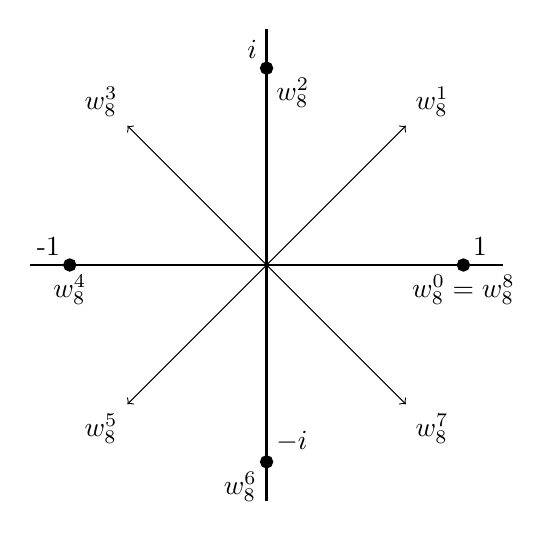
\begin{tikzpicture}
    \draw[thick](0, 0) -- (0, 3); 
    \draw[thick](0, 0) -- (3, 0);
    \draw[thick](0, 0) -- (0, -3);
    \draw[thick](0, 0) -- (-3, 0);

    \draw[thick,fill=black](2.5, 0)circle[radius=2pt];
    \draw[thick,fill=black](0, -2.5)circle[radius=2pt];
    \draw[thick, fill=black](0, 2.5)circle[radius=2pt];
    \draw[thick,fill=black](-2.5, 0)circle[radius=2pt];

    \draw(2.5, 0)node[anchor=south west]{1};
    \draw(-2.5, 0)node[anchor=south east]{-1};
    \draw(0, 2.5)node[anchor=south east]{$i$};
    \draw(0, -2.5)node[anchor=south west]{$-i$};

    \draw [->] (0, 0) -- (2.5, 0)node[anchor=north]{$w_8^0 = w_8^8$};
    \draw [->] (0, 0) -- (-2.5, 0)node[anchor=north]{$w_8^4$};
    \draw [->] (0, 0) -- (0, 2.5)node[anchor=north west]{$w_8^2$};
    \draw [->] (0, 0) -- (0, -2.5)node[anchor=north east]{$w_8^6$};

    \draw [->] (0, 0) -- ({2.5*cos(45)}, {2.5*sin(45)})node[anchor=south west]{$w_8^1$};
    \draw [->] (0, 0) -- ({-2.5*cos(45)}, {2.5*sin(45)})node[anchor=south east]{$w_8^3$};
    \draw [->] (0, 0) -- ({-2.5*cos(45)}, {-2.5*sin(45)})node[anchor=north east]{$w_8^5$};
    \draw [->] (0, 0) -- ({2.5*cos(45)}, {-2.5*sin(45)})node[anchor=north west]{$w_8^7$};
\end{tikzpicture}
\\
위 그래프는 $w_8 = e^{2 \pi i /8}$일 때, $w_8^0, w_8^1, ... w_8^7$을 복소평면에 표현한 것이다. 
\\
$w_n = e^{2 \pi i/n}$는 1의 n제곱근의 principal이다. 모든 n제곱근은 $w_n$의 승수 형태이다. 
\\
n개의 1의 n제곱근은 다음과 같다. 
$$
w_n^0, w_n^1, ... , w_n^{n-1}.
$$
이 군은 곱셈형태에 대해 지수가 더해진다. 실수에서 자기 곱셈형태는 지수 +1이 되듯이 말이다. $a*a = a^{1+1}=a^2$
$w_n^n = w_n^0 = 1$은 다음을 뜻한다. $w_n^j w_n^k = w_n^{j+k} = w_n^{(j+k)\mod{n}}$
단, 단순 곱을 수행할 수는 없다. 예로, 실수에선 종종 이런식으로 이해하기도 한다. $(a^{b})^{1/2} = a^{b/2}$
그러나 이 군에서는 정수에 대해서만 수행할 수 있다. 따라서 다음 명제는 참이다. $e^{2 \pi i/n} \ne (e^{2 \pi i})^{1/n}.$
\vspace{5mm}
\\
\textbf{\textit{Lemma (Cancellation lemma)}}
\\
모든 정수 $n \ge 0, k \ge 0, d > 0$에 대하여 다음을 만족한다. 
$$w_{dn}^{dk} = w_n^k$$
\vspace{5mm}
\textbf{\textit{증명}}
\begin{align*}
    w_{dn}^{dk} &= (e^{2 \pi i/dn})^{dk}\\
    &=(e^{2 \pi i/n})^k\\
    &= w_n^k.
\end{align*}
\vspace{5mm}
\\
\textbf{\textit{딸림 정리}} 짝수 $n > 0$에 대하여 다음을 만족한다. 
$$
w_n^{n/2} = e^{2 (n/2) \pi i / n} = e^{\pi i} =  w_2 = -1.
$$
$n/2$가 임의의 정수이므로 덧셈이 가능하다. 
\vspace{5mm}
\\
\textbf{\textit{Lemma (Halving lemma)}}
\\
$n$이 짝수일 때, $n$개의 1의 $n$제곱근은 그 제곱이 $n/2$개의 1의 $n/2$제곱근과 같다. 
\vspace{5mm}
\\
\textbf{\textit{증명}}
\\
cancellation lemma에 따라 다음을 만족한다. $(w_n^k)^2 = w_{n/2}^k$,k는 정수. 
만약 $n$개의 1의 n제곱근들을 제곱한다면, $n/2$개의 1의 $n/2$제곱근들이 각각 2개씩 존재하는 형태가 될것이다. 
\begin{align*}
    (w_n^{k+n/2})^2 &= w_n^{2k+n}\\
    &=w_n^n w_n^{2k}\\
    &=w_n^{2k}\\
    &=(w_n^k)^2.
\end{align*}
따라서, $(w_n^{k+n/2})^2 = (w_n^k)^2$이므로 $n$개의 제곱근을 제곱하였을 때 $k=0, ... n/2-1$과 $k=n/2, ... n-1$의 값이 겹치게된다. 
$n$개의 1의 n제곱근의 제곱은 n/2이후로 반복된 패턴을 가지며, $(w_n^k)^2 = w_{n/2}^k$이므로 $n/2$개의 1의 $n/2$ 제곱근들이 각각 두개씩 존재하는 형태이다. 
복소평면에서 그렸던 그래프를 빌어 이야기하자면, $w_n^k = e^{2 k \pi i /n}$가 복소평면을 피자판처럼 n개 분할하였을 때 k 번째 직선이라면, 
$(w_n^k)^2 = w_n^{2k} = w_{n/2}^k$ 이므로 복소평면을 $n/2$ 개의 피자판으로 쪼갰을 때, k 번째 즉 이전 직선에서 정확히 두배 더 넓은 각을 가지는 
직선이 되는 것이다. 해당 직선은 2배로 넓은 각을 형성하니 한번 더 원점을 기준으로 도는 형태가 되어 같은 방향으로 두 번씩 발생할것이다. 
\\
추가적인 정보를 위한 사람들을 위해 복소수 기초를 다루는 유튜브 강의는 다음 링크로 남겨둔다. 필요한 부분만 참고하시길. 
\href{https://www.youtube.com/watch?v=-dOliRrDQ8k}{링크}
\\
\\
\vspace{5mm}
\Large{The DFT}
\normalsize
\\
다음 다항식이 있다.
$$
A(x) = \sum_{j=0}^{n-1}a_jx^j.
$$
이 때 $w_n^i$가 x의 값이 대안이 될 수 있다. $w_n^i$를 대입하였을 때 결과값을 $y$라 하자.
\begin{align*}
    y_k &= A(w_n^k)\\
    &=\sum_{j=0}^{n-1}a_jw_n^{kj}.
\end{align*}
이 때, $y =(y_0, y_1, ... , y_{n-1})$를 계수 벡터 $a=(a_0, a_1, ... ,a_{n-1})$의 DFT라고 한다.   
$y=DFT_n(a)$라고도 할 수 있다.
\\
\\
\vspace{5mm}
\Large{The FFT}
\normalsize
\\
fast fourier transform(FFT)는 1의 n제곱근의 특성을 이용하여 $\Theta (n)$ 복잡도에 $DFT_n(a)$를 구한다. 
차수 n은 2의 제곱승으로 맞춰줄것이다. 차수가 2의 제곱승이 아닌 다항식을 처리하는 알고리즘이 존재하지만 말이다. 
\\
FFT는 분할정복 기법을 이용하는데 다항식 $A$의 홀수인덱스, 짝수인덱스를 분리해서 사용한다. 
그리고 이 방법을 통해 다음과 같은 식을 유도할 수 있다. 
\begin{align*}
    &A^{[0]}(x) = a_0 + a_2x + a_4x^2 + ... + a_{n-2}x^{n/2-1}\\
    &A^{[1]}(x) = a_1 + a_3x + a_5x^2 + ... + a_{n-1}x^{n/2-1}\\
    &A(x)=A^{[0]}(x^2)+xA^{[1]}(x^2).\tag{1}
\end{align*}
이 때 다항식 $A(x)$, at $w_n^0, w_n^1, ... , w_n^{n-1}$ 값을 구하는 문제가 된다. 
이 문제는 다음과 동치인 문제이다. 
\\
1. n/2차 항인 $A^{[0]}(x)$와 $A^{[1]}(x)$의 값을 구한다. 이때 x는 다음과 같다. 
\[
    (w_n^0)^2, (w_n^1)^2, ..., (w_n^{n-1})^2\tag{2}
\]
\\
2. 식 $(1)$ 과 두 다항식의 결과값을 이용하여 $A(x)$를 도출한다. 
\\
halving lemma에 따라, 수식 $(2)$에서 $(w_n^i)^2 = (w_n^{n/2+i})^2$이다. 
따라서 우리는 $A^{[0]}, A^{[1]}$의 $n/2$개 이후의 값은 초반 $n/2$가 반복되는 것이다.
그러면 다음과 같이 서술할 수 있다. $A^{[0]}(x), A^{[1]}(x)$의 값을 $(w_n^0)^2, (w_n^1)^2, ... , (w_n^{n/2-1})^2$의 위치에서 구하고 
그 결과를 두배한 것 과 같다. 그러면 문제는 다음과 같은 부분문제를 갖게된다. 
\\
\textbf{Origin Problem}
\\
n차 항인 $A(x)$의 at $w_n^0, w_n^1, ... , w_n^{n-1}$의 값을 구하라. 
\\
\textbf{Sub Problem}
\\
n/2차 항인 $A^{[0]}(x), A^{[1]}(x)$의 at $(w_n^0)^2, (w_n^1)^2, ... , (w_n^{n/2-1})^2$의 값을 구하라.
\\
\textbf{merging}
\\
n/2차 항인 $A^{[0]}(x)$의 y벡터가 $y^{[0]}$, $A^{[1]}(x)$의 y 벡터가 $y^{[1]}$라 하자. 
이 때, $y_k = y_k^{[0]} + w_n^k y_k^{[1]}$ 그리고 $y_{n/2+k} = y_k^{[0]} - w_n^k y_k^{[1]}$ 이다. 
\pagebreak
\\
아래는 이 접근법을 코드로 작성해본 것이다. 
\begin{lstlisting}
vector<int> FFT(vector<int> a)
{
    int n = a.size();
    if ( n == 1) return a;

    w = E; // where E = e^(2 pi i)
    w2 = 1;

    vector<int> azero, aone;

    for (int i = 0; i<n/2; i++)
    {
        azero.push_back(a[i]);
        aone.push_back(a[n/2 + i]);
    }
    vector<int> yzero, yone;
    yzero = FFT(azero);
    yone = FFT(yone);

    vector<int> ret(n);
    for (int i=0; i<n/2; i++)
    {
        ret[i] = yzero[i] + w2*yone[i];
        ret[i+n/2] = yzero[i] - w2*yone[i];
        w2*=w;
    }
    return ret;
}
\end{lstlisting}
\textbf{merging} 파트를 보자. $23 \tilde 24$ Line에 위치하고 있다. 
$y_k = y_k^{[0]} + w_n^k y_k^{[1]}$의 정당성을 보자. 
\begin{align*}
    y_k &= y_k^{[0]} + w_n^k y_k^{[1]}\\
    &=A^{[0]}(w_n^{2k}) + w_n^kA^{[1]}(w_n^{2k})\\
    &=A(w_n^k) &\text{수식 (1) 에 의해 }
\end{align*}
$y_{k+n/2} = y_k^{[0]} - w_n^k y_k^{[1]}$의 정당성을 보자. 
\begin{align*}
    y_{n/2+k} &= y_k^{[0]} - w_n^k y_k^{[1]}\\
    &=A^{[0]}(w_n^{2k}) + w_n^{n/2+k}A^{[1]}(w_n^{2k})\\
    &=A^{[0]}(w_n^{2k+n}) + w_n^{n/2+k}A^{[1]}(w_n^{2k+n})\\
    &=A(w_n^{n/2+k}) &\text{수식 (1) 에 의해 }
\end{align*}
\pagebreak
\subsection{효율적인 FFT 구현}

\begin{lstlisting}
vector<int> FFT(vector<int> a)
{
    int n = a.size();
    if ( n == 1) return a;

    w = E; // where E = e^(2 pi i)
    w2 = 1;

    vector<int> azero, aone;

    for (int i = 0; i<n/2; i++)
    {
        azero.push_back(a[i]);
        aone.push_back(a[n/2 + i]);
    }
    vector<int> yzero, yone;
    yzero = FFT(azero);
    yone = FFT(yone);

    vector<int> ret(n);
    for (int i=0; i<n/2; i++)
    {
        ret[i] = yzero[i] + w2*yone[i];
        ret[i+n/2] = yzero[i] - w2*yone[i];
        w2*=w;
    }
    return ret;
}
\end{lstlisting}
\end{document}